\section{Reproducing Kernel Hilbert Space} 

\subsection{Hilbert Space}
We can define a Hilbert space $\mathcal{H}$ an inner product space that is complete and separable with respect to the norm defined by inner product.
An example of a defined norm in Hilbert space (i.e, the space $L_2$ of square integrable functions) can be 
\begin{equation*}
    \parallel f \parallel = \left(\int_a^b f^2(t)dx\right)^\frac{1}{2}.
\end{equation*}
A normed space is a vector space $N$ on which a norm is defined. A nonnegative function $\parallel\cdot\parallel$ is a norm if and only if $\forall f,g\in N$ and $\alpha\in\mathbb{R}$:
\begin{itemize}
    \item $\parallel f \parallel \geq 0$ and $\parallel f\parallel=0$ iff $f=0$;
    \item $\parallel f+g \parallel \leq \parallel f \parallel + \parallel g \parallel$;
    \item $\parallel \alpha f\parallel=\mid \alpha \mid \parallel f \parallel$
\end{itemize}
Examples of inner product $<a,b>$ in a Hilbert space are
\begin{itemize}
    \item a usual dot product: $<a,b>=a'b=\sum_i a_i b_i$.
    \item a kernel product: $<a,b>=k(a,b)=\psi(a)'\psi(b)$, where $\psi(a)$ may have infinite dimensions.
\end{itemize} 

\subsection{Introduction to Kernel}
\subsubsection{Feature map}
The motivation of kernel method is simple. Imagine there are some blue dots and red dots on a vector space $\mathcal{R}^2$ and 
we want to separate them by color. As it shows in the left hand side figure, it is difficult to divide them through a straight 
line. However, we may be able to separate them easily by mapping each dot into a high-dimension feature space. The figure below 
shows how feature map works:
\begin{figure}[H]
    \centering
    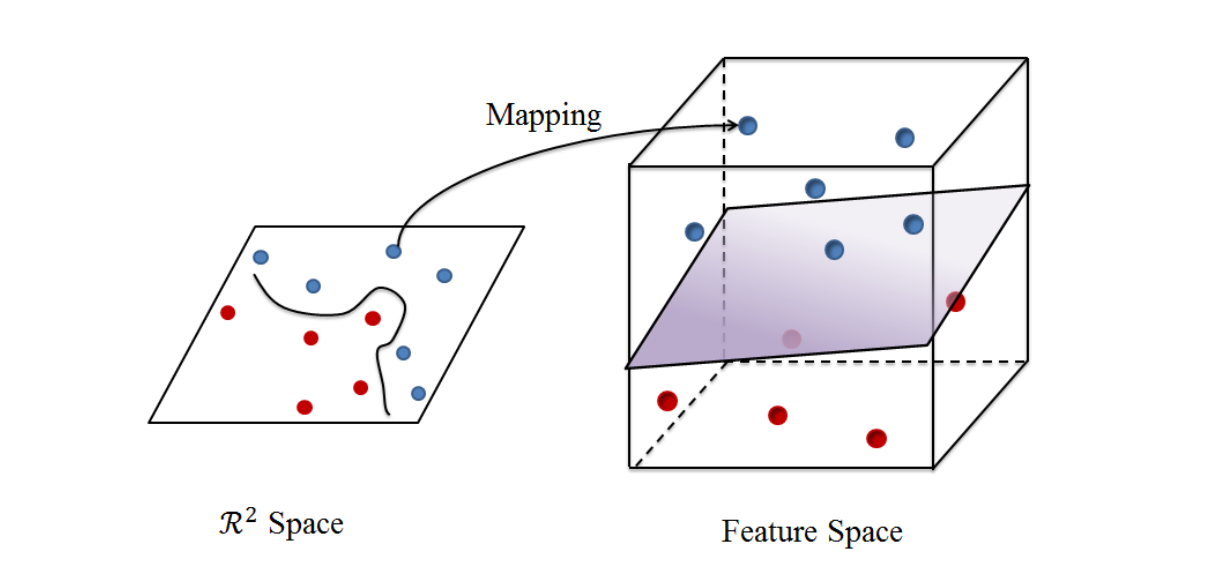
\includegraphics[width=0.7\textwidth]{Mapping}
\end{figure}
Let's now use a simple example to illustrate the idea of feature map. 
we set two vectors $\textbf{x}=\begin{bmatrix}x_1&x_2\end{bmatrix}$ and $\textbf{y}=\begin{bmatrix}y_1&y_2\end{bmatrix}$ in a two-dimension space.
Tow functions $\phi(x)$ and $\phi(y)$ are defined as:
\begin{equation*}
    \phi(x)=\begin{bmatrix}
        x_1x_1&x_1x_2&x_2x_1&x_2x_2
    \end{bmatrix}
\end{equation*}
\begin{equation*}
    \phi(y)=\begin{bmatrix}
        y_1y_1&y_1y_2&y_2y_1&y_2y_2
    \end{bmatrix}
\end{equation*}
We are now successfully mapping them into a four-dimension feature space. 
To write the above example in a general form of linear regression, we first set an equation where $\phi(\cdot)\in\mathcal{R}^m$ and $\phi(x)$ is defined as the mapping function. Note that we assume there is a linear relation between $y$ and $\phi(x)$:
\begin{align}
    y&=\phi(x)^\top w \notag\\
     &= \begin{bmatrix}
        \phi_1(x)\cdots\phi_m(x)
        \end{bmatrix} w
\end{align}
$Y$ and $\Phi$ in generalization is defined by:
\begin{equation}
    Y=\begin{bmatrix}
         y_1&\cdots&y_n
      \end{bmatrix}^\top 
\end{equation}
\begin{align}
    \Phi&=\begin{bmatrix}
           \phi(x_1)&\cdots&\phi(x_n) 
          \end{bmatrix}^\top \notag\\
        &=\begin{bmatrix}
           \phi_1(x_1)&\cdots&\phi_m(x_1)\\
           \vdots&\vdots&\vdots \\
           \phi_1(x_n)&\cdots&\phi_m(x_n)
          \end{bmatrix}
\end{align}
Recall the regularized risk minimization problem of ridge regression. In this case, it can be re-written as:
\begin{align*}
    w{*}&=\underset{w}{\operateorname{argmin}}\sum_{i=1}^n(y_i-\phi(x_i)^\top w)^2+\lambda\parallel w \parallel_2^2\\
      &=\underset{w}{\operateorname{argmin}}\parallel Y-\Phi w\parallel_2^2+\lambda\parallel w\parallel_2^2
\end{align*}
The least-square solution can also be re-defined by:
\begin{equation}
    w{*}=(\Phi^\top\Phi+\lambda I)^{-1}\Phi^\top Y
\end{equation}
Then we replace $w{*}$ with $(\Phi^\top \Phi+\lambda I)^{-1}\Phi^\top$ in $y=\phi(x)^\top w$, we get:
\begin{align}
    y_w{*} (x)&=\phi(x)^\top w{*}\notag\\
            &=\phi(x)^\top(\Phi^\top \Phi+\lambda I)^{-1}\Phi^\top Y\notag\\
            &=\underbrace{\phi(x)^\top \Phi^\top}_\text{$1\times n$}(\underbrace{\Phi\Phi^\top}_\text{$n\times n$}+\lambda I)^{-1}Y\\
            &\text{using that} (\Phi^\top \Phi+\lambda I)^{-1}\Phi^\top=\Phi^\top(\Phi\Phi^\top+\lambda I)^{-1}\notag
\end{align}


\subsubsection{Kernel Method}
In most of the cases, it is surprisingly difficult to know and calculate the feature function after mapping. We want to avoid computing $\phi(x)$ in a explicit way, 
especially when $m$ is very large. Therefore, we define a kernel function:
\begin{equation*}
    [\Phi\Phi^\top]_{i,j}=\phi(x_i)^\top \phi(x_j)=K(x_i,x_j)
\end{equation*}
\begin{equation}
    [\phi(x)^\top\Phi^\top]_j=\phi(x)^\top\phi(x_j)=K(x,x_j)
\end{equation}
This is simply the intuition of using the kernel method. For example, the Gaussian kernel is
\begin{equation*}
    k(x_i, x_j) = e^\frac{-\parallel x_i - x_j \parallel}{\sigma^2},
\end{equation*}
Gaussian kernel meaning the similarity between two points where $\parallel x_i - x_j \parallel$ is the Euclidean distance between $x_i$ and $x_j$, and $\sigma^2 \in \mathbb{R}^+$ is the bandwidth of the kernel function, and it satisfies the 
following properties:\\
for $k: \mathcal{X} \times \mathcal{X} \rightarrow \mathbb{R}$ is a kernel if
\begin{itemize}
    \item $k$ is symmetric: $k(x,y) = k(y,x)$.
    \item $k$ is positive semi-definite, meaning that $\sum_{i} \sum_{j} \alpha_i \alpha_j k(x_i,x_j)\geq0, \forall \alpha_i, \alpha_j \in \mathbb{R}, x \in \mathbb{R}^\mathbb{D}, \mathbb{D} \in \mathbb{Z}^+$. 
    \item We define the corresponding kernel matrix as the matrix $K$ with entries $k_{ij}=k(x_i,x_j)$, the sencond property of $k$ is equivalent to saying that $\textbf{a}'K \textbf{a}\geq 0$.
\end{itemize}
Now we can define a function k: $\mathcal{X} \times \mathcal{X}  \rightarrow \mathbb{R}$ is a kernel if and 
only if there exists a Hilbert space $\mathcal{H}$ and a map $\phi: \mathcal{X}\rightarrow\mathcal{H}$ such that $k(x,y)=<\phi(x),\phi(y)>$. 
\\ \\
Recall the simple example above, instead of computing the inner product of $<\phi(x),\phi(y)>$, we can define 
a corresponding kernel function $K(\textbf{x},\textbf{y})=<\textbf{x},\textbf{y}>^2$. It can be easily proofed that $K(\textbf{x},\textbf{y})$ is the same as $<\phi(\textbf{x}),\phi(\textbf{y})>$:
\begin{align*}
    K(\textbf{x},\textbf{y})&=<\textbf{x},\textbf{y}>^2\\
                            &=(x_1y_1+x_2y_2)^2\\
                            &=x_1^2y_1^2+2x_1y_2x_2y_1+x_2^2y_2^2\\
                            &=<\phi(\textbf{x}),\phi(\textbf{y})>
\end{align*}

\subsection{Reproducing Kernel Hilbert Space}
Consider a Hilbert space $\mathcal{H}$ full of real-valued functions from $\mathcal{X}$ to $\mathbb{R}$, and a mapping $\Phi: \mathcal{X}\rightarrow\mathbb{R}^\chi$ defined as $x\rightarrow\Phi(x)=k_x=k(\cdot , x)$. A function $k:\mathcal{X}\times\mathcal{X}\rightarrow\mathbb{R}$ is a 
reproducing kernel of $\mathcal{H}$, and $\mathcal{H}$ is a reproducing kernel Hilbert space, if:
\begin{itemize}
    \item $\forall x \in\mathcal{X}$, $k(\cdot, x)\in\mathcal{H}$,
    \item $\forall x \in\mathcal{X}$, $f\in\mathcal{H}$, $<f(\cdot),k(\cdot,x)>_\mathcal{H}=f(x)$, which is the reproducing property.
\end{itemize}
To be more intuitively, a Reproducing Kernel Hilbert Space is a Hilbert space $\mathcal{H}$ with a reproducing kernel whose span is dense in $\mathcal{H}$. Equivalently, a RKHS can be defined as a Hilbert space of valid functions  with all evaluation functionals bounded and linear. 

\subsection{Representer Theorem}
In the previous section, we have learned that there is always a pair of $(\mathcal{X},k)$ as a Hilbert space or a subset of that space whenever the input domain $\mathcal{X}$ exists. Such a fact means that we are able to study the various data structures in Hilbert spaces. 
In practical world, however, it is extremely difficult to study many popular kernels since their Hilbert spaces is known to be infinite-dimensional in almost every case. Especially for the purpose of machine learning, we usually prefer solve an optimization problem in a finite-dimensinal space. 
\\ \\
This is where the representer therom useful. It contributes to simplify the regularized risk-minimization problem by reducing the infinite-dimensional space to finite-dimensional vector of optimal coefficients, and provide provisions for kernels in training data in machine learning.
\\ \\
(not neccessary)To illustrate the representer theroem, we first set a paired observations $(x_1,y_1),\cdots,(x_n,y_n)$ to be either classification or regression Loss function. 
\begin{itemize}
    \item Classification: $L_y(f(x_1),\cdots,f(x_n))=\sum_{i=1}^n \mathbb{I}_{y_i f(x_i)\leq0}$
    \item Regression: $L_y(f(x_1),\cdots,f(x_n))=\sum_{i=1}^n(y_i-f(x_i))^2$
\end{itemize}
(net neccessary)
\\ \\
With assumptions here!!!!
In the RKHS $\mathcal{H}$, we can find the function $f^{*}$ satisfying:
\begin{equation*}
    \mathcal{J}(f^{*})=\underset{f\in\mathcal{H}}{min}\mathcal{J}(f),
\end{equation*}
where 
\begin{equation*}
    \mathcal{J}(f)=L_y(f(x_1),\cdots,f(x_n))+\Omega(\parallel f \parallel_\mathcal{H}^2).
\end{equation*}
Note that $\Omega$ is non-decreasing regularizer and $y$ is a vector of $y_i$. 
\\ \\
The representer theorem is that the solution to $\underset{f\in\mathcal{H}}{min}[L_y(f(x_1),\cdots,f(x_n))+\Omega(\parallel f \parallel_\mathcal{H}^2)]$ can 
be written in a simpler version, which takes the form $f^{*}=\sum_{i=1}^n\alpha_i k(x_i,\cdot)$. If $\Omega$ is strictly increasing, all solutions apply to this form. 


\subsection{Example using representer theroem--Kernel ridge regression}
In the simplest form of machine learning, in order to predict $x$, the algorithm collects the samples in the training set $\mathcal{X}$ that are similar to $x$, 
and then take the weighted value of these samples as the predict value of $x$. Here comes the questions:
\begin{itemize}
    \item How to measure the similarity between samples?
    \item How to weight the value of each sample?
\end{itemize} 
In general, the higher the similarity of the sample to our point of interest $x$, the more the sampling weights. To evaluate the similarity between two observations, 
a kernel is defined as a function of two input patterns $k(x_i, x_j)$, mapping onto a real-valued output.
\\ \\
From the similarity-based point of view, the use of kernels for regression can be described in two stages. We set $y_i \in \mathbb{R}$ as dependent variable, 
and $x_i$ as a $1 \times D$ vector $x_i \in \mathbb{R}^D$ of covariate values. Assume that $(y_i, x_i)$ where $i = 1, \dots, N$ is i.i.d. We first define a target function $y=g(x)$ and assume that in a space of functions, there exists 
a function that can estimate $y=g(x)$ well. The target function can be represented by
\begin{align}
    g(x)&= <\textbf{w},\Phi(x)>\notag\\
        &=\sum_{i=1}^N w_i k(\cdot,x_i).
\end{align}
We can solve this linear regression problem by least square $\underset{w\in\mathbb{R}^d}{minimize}\frac{1}{n}\sum_{i=1}^n(y_i-<\phi(x_i),w>^)2$ in the feature space with a mapping $\phi: \mathcal{X}\rightarrow\mathbb{R}^d$. Luckily, the 
representer theorem already tells us that the least squared problem always has a solution of the form $w^{*}=\sum_{j=1}^n\alpha_j\phi(x_j)$. We them plug it into the objective function and use the repreducing property of RKHS, and get:
\begin{align*}
    \underset{w\in\mathbb{R}^d}{minimize}\frac{1}{n}\sum_{i=1}^n(y_i-<\phi(x_i),w>^2)&\Leftrightarrow\\
                                                                                     &\underset{\alpha\in\mathbb{R}^n}{minimize}\frac{1}{n}\sum_{i=1}^n(y_i-\sum_{j=1}^n\alpha_j<\phi(x_i),\phi(x_j)>)^2\\
                                                                                     &\underset{\alpha\in\mathbb{R}^n}{minimize}\frac{1}{n}\sum_{i=1}^n(y_i-\sum_{j=1}^n\alpha_j k(x_i,x_j))^2\\
                                                        \text{in matrix notation:}  &\underset{\alpha\in\mathbb{R}^n}{minimize}\frac{1}{n}\parallel Y-K\alpha\parallel^2
\end{align*}
\\ \\
A perfect solution to estimate N parameters for N observations would be choosing $\hat{w}=K^{-1}y$. However, such a fit could result in extremely high variance. Therefore, we impose an addtional assumption 
that a smoother curve with less oscillations is prefered. We then utilize regularization to simplify the function and satisfy the additional assumption by adding a penalty term $\lambda$ in 
the second stage. 
\\ \\
Use features of $\phi(x_i)$ in the place of $x_i$, a ridge regression with kernel based can be defined:
\begin{equation}
    w^*=\underset{w\in\mathcal{H}}{argmin}\left(\sum_{i=1}^n(y_i-<w,\phi(x_i)>_\mathcal{H})^2+\lambda\parallel w\parallel_\mathcal{H}^2\right)
\end{equation}
Remember the corresponding kernel matrix as the matrix $K$ with entries $k_{ij}=k(x_i,x_j)$ is equivalent to saying that $\textbf{a}'K \textbf{a}\geq 0$, we can then rewrite the kernel ridge regression as:
\begin{align}
    \sum_{i=1}^n(y_i-<w,\phi(x_i)>_\mathcal{H})^2+\lambda\parallel w\parallel_\mathcal{H}^2 \notag\\
    &\Leftrightarrow\parallel y_i-K \alpha\parallel^2+\lambda \textbf{a}' K\textbf{a}.
\end{align}
By differentiation and setting the equation $(9)$ to zero, we get:
\begin{equation}
    \alpha^{*}=(K+\lambda I_n)^{-1}y.
\end{equation}